%% IEEE Transactions on Signal Processing version (IEEEtran journal, two columns).
%% The text is shared with the Signal Processing version: ../paper/body.tex.
\documentclass[journal]{IEEEtran}

\usepackage{amsmath,amssymb,amsfonts,amsthm}
\usepackage{graphicx}
\usepackage{booktabs}
\usepackage{array}
\usepackage{xcolor}
\usepackage{algorithm}
\usepackage{algpseudocode}
\usepackage{tikz}
\usetikzlibrary{arrows.meta,positioning,calc}
\usepackage{cite}
\usepackage[hidelinks]{hyperref}
\graphicspath{{../paper/figs/}}

\newif\ifsp \spfalse
%% Macros and theorem environments shared by the SP (elsarticle) and TSP (IEEEtran) versions.
\newtheorem{theorem}{Theorem}
\newtheorem{proposition}{Proposition}
\newtheorem{lemma}{Lemma}
\newtheorem{corollary}{Corollary}
\theoremstyle{definition}
\newtheorem{definition}{Definition}
\newtheorem{remark}{Remark}

\newcommand{\Ts}{T_{\mathrm{s}}}
\newcommand{\cd}{c_{\mathrm{d}}}
\newcommand{\sd}{s_{\mathrm{d}}}
\newcommand{\ulo}{u_{\mathrm{lo}}}
\newcommand{\uhi}{u_{\mathrm{hi}}}
\newcommand{\xlo}{\xi_{\mathrm{lo}}}
\newcommand{\xhi}{\xi_{\mathrm{hi}}}
\newcommand{\gh}{\hat g}
\newcommand{\Hh}{\hat H}
\newcommand{\Op}[2]{{}^{\mathrm{#1}}\!\Delta^{#2}}
\newcommand{\WA}{W_{\mathrm A}}
\newcommand{\WB}{W_{\mathrm B}}
\newcommand{\WD}{W_{\mathrm D}}
\newcommand{\WE}{W_{\mathrm E}}
\newcommand{\Beta}{\mathrm{B}}
\newcommand{\eps}{\varepsilon}
\newcommand{\pending}[1]{\textcolor{red}{[#1]}}


%% References to labels of the main text: plain in the main text, prefixed M- in a supplement
\providecommand{\mref}[1]{\ref{#1}}
\providecommand{\meqref}[1]{\eqref{#1}}
%% Citation lists: the full list in the TSP version, a shorter one in the SP version (page limit)
\providecommand{\citesp}[2]{\ifsp\cite{#2}\else\cite{#1}\fi}

\newcommand{\partsdir}{../paper/parts/}
\newcommand{\proofref}[1]{Appendix~\ref{#1}}
\newcommand{\tabfont}{\scriptsize}
\newcommand{\colfigwidth}{\columnwidth}

\begin{document}

\title{Variable-Order Fractional Operators from Fixed-Pole Banks: Definition by Structure, Error Guarantees, and Order Tracking}

\author{First~Author and Second~Author% TODO: names and affiliations
\thanks{\pending{TODO: affiliations, e-mail addresses, funding.}}}

\maketitle

\begin{abstract}
Variable-order (VO) fractional operators have several inequivalent definitions that differ in how past orders enter the memory, and it is unclear which definition a finite-dimensional realization implements when it switches coefficients as the order varies. We show that an exact switching state map exists only between similar realizations, so realizations whose poles move with the order cannot implement the A- or B-type Gr\"unwald--Letnikov (GL) definitions under switching. A Beta-integral representation instead realizes the GL weights with order-independent poles. With the order in the output weights the bank is the A-type, with it in the input weights the B-type, for every order sequence; inverting it gives the recursive D- and E-types with exact duality, all at $O(K)$ cost. In the $\ell^1$ and $\ell^\infty$ norms the relative operator error of the forward types never exceeds the relative weight error. The construction extends to every kernel family that is completely monotone in the lag, with $K=O(\ln(1/\eps)\ln(R/\eps))$ common poles for tolerance $\eps$ and memory $R$. A fit-free design rule met all 400 specifications of a sealed holdout. For tracking a time-varying order, the A-type bank makes an exact grid filter affordable, and a B-type extended Kalman filter on the bank comes within 6\,\% of the causal Bayesian Cram\'er--Rao bound. On measured lithium-ion drive cycles, running a fitted VO model with the other definition increased its held-out error in 51 of 56 cases, while the bank matched the literal GL sum to $3\times10^{-6}$ at a fixed cost.
\end{abstract}

\begin{IEEEkeywords}
Variable-order fractional calculus, Gr\"unwald--Letnikov, fixed-pole approximation, completely monotone kernels, order tracking, posterior Cram\'er--Rao bound, lithium-ion battery.
\end{IEEEkeywords}

%% =====================================================================
%% Main text shared by the SP version (paper/main.tex) and the TSP version (paper_tsp/main.tex).
%% \ifsp selects what the SP version moves to its supplement.
\section{Introduction}\label{sec:intro}

\IEEEPARstart{F}{ractional-order} operators describe systems whose memory decays as a power law. When the exponent itself changes in time, the natural model is a variable-order (VO) operator with order $\alpha(t)$~\citesp{samko1993,lorenzo2002,sun2019,patnaik2020}{samko1993,lorenzo2002}. Unlike the constant-order case, the generalization is not unique: different ways of letting the order enter the memory give operators that coincide for constant order but differ as soon as the order changes~\citesp{lorenzo2002,valerio2011,garrappa2021}{lorenzo2002,valerio2011}. For Gr\"unwald--Letnikov (GL) operators, Sierociuk et al.\ use four types~\citesp{sierociuk2015amm,sierociuk2015cssp,malesza2016,sierociuk2020}{sierociuk2015amm,sierociuk2015cssp,sierociuk2020}. The A-type weights the whole history with the current order; the B-type weights each past sample with the order that was active when the sample entered; the recursive D- and E-types are the inverses of the A- and B-types of opposite order. After a single switch these definitions differ by as much as the output itself, so the definition is part of the model.

Practical realizations are finite-dimensional. Constant-order operators are approximated by rational transfer functions, most often by Oustaloup's recursive distribution of poles and zeros~\cite{oustaloup2000} and related schemes~\citesp{charef1992,vinagre2000}{charef1992}, whose poles move with the order. Fixed-pole approximations exist for constant orders~\citesp{wei2016,wei2019,wei2021}{wei2021}, and diffusive and sum-of-exponentials representations lead to fixed nodes~\citesp{montseny1998,trigeassou2012,baffet2017,jiang2017,diethelm2023}{montseny1998,diethelm2023}. When the order varies, a constant-order realization is switched between orders, by switching circuits~\citesp{sierociuk2015amm,macias2020,zhou2019}{sierociuk2015amm,macias2020} or by changing coefficients while keeping the state (a ``hot swap''). Direct GL convolutions with current-order weights~\cite{tolba2020,oziablo2020} are A-type operators whose cost grows with the memory. Order-independent exponents have been used for the A-type VO Caputo derivative in fast solvers~\citesp{zhang2022esa,zhang2022fast,huang2022unified}{zhang2022fast}, without the B-, D- or E-types, a design rule over the order range, or hardware. Transients after coefficient changes in recursive filters are a classical topic~\citesp{zetterberg1988,valimaki1998}{zetterberg1988}, but none of these lines asks which VO definition a switched realization implements.



\ifsp A table in the Supplementary Material\else\input{\partsdir tab_related}

Table~\ref{tab:related}\fi{} summarizes how existing realizations treat a varying order. This paper answers two questions for GL operators of order $-1<\alpha<1$ and, more generally, for kernel families that are completely monotone in the lag: which VO definition does a finite-dimensional realization implement for an arbitrary order sequence, and can its structure select the definition at no extra cost? The contributions are:
\begin{enumerate}
\item \emph{Necessity:} an exact switching state map exists only between similar realizations (Theorem~\ref{thm:necessity}); moving-pole realizations cannot implement the A- or B-type at a switch.
\item \emph{Definition by structure:} a Beta-integral representation gives a discrete bank with order-independent poles that realizes the A-type with the order in the output weights and the B-type with it in the input weights, for every order sequence (Proposition~\ref{prop:structure}); inverting it gives the D- and E-types with exact duality (Proposition~\ref{prop:inverse}).
\item \emph{Guarantees:} the relative operator error of the forward types never exceeds the relative weight error in $\ell^1$ and $\ell^\infty$ (Theorem~\ref{thm:opnorm}); the results hold for every completely monotone kernel family, with explicit constants for GL (Theorem~\ref{thm:cm}); a fit-free rule sizes the bank, and the inverse is stable if and only if a realized DC gain is positive (Proposition~\ref{prop:stability}).
\item \emph{Order tracking:} the A-type bank has order-independent regressors, which makes an exact grid filter affordable; we derive the posterior Cram\'er--Rao bound and compare the estimators with it (Sect.~\ref{sec:track}).
\item \emph{Measured data:} on lithium-ion drive cycles, the definition and the memory length decide the error of a fitted VO model, and one bank fits and runs both definitions at a fixed cost (Sect.~\ref{sec:battery}).
\end{enumerate}
A fixed-point core realizes all four types and was verified bit-exact on an FPGA board (Sect.~\ref{sec:hw}). Proofs are in \ifsp the Supplementary Material\else the Appendix\fi; continuous-time results and implementation details are in the Supplementary Material; code, seeds and results are public.

%% =====================================================================
\section{Variable-order GL operators}\label{sec:prelim}

Let $\Ts$ be the sampling period and $\alpha_n\in(-1,1)$ the order at sample $n\ge0$; $\alpha>0$ is a derivative, $\alpha<0$ an integral, and signals vanish for $n<0$. With
\begin{equation}
w_r(a)=(-1)^r\tbinom{a}{r}=w_{r-1}(a)\tfrac{r-1-a}{r},\quad g_r(a)=\Ts^{-a}w_r(a),\label{eq:glw}
\end{equation}
with $w_0=1$, the four types are~\cite{sierociuk2015amm,sierociuk2015cssp,sierociuk2020}
\begin{align}
\big(\Op{A}{\alpha}x\big)_n &= \textstyle\sum_{r=0}^{n} g_r(\alpha_n)\,x_{n-r}, \label{eq:A}\\
\big(\Op{B}{\alpha}x\big)_n &= \textstyle\sum_{r=0}^{n} g_r(\alpha_{n-r})\,x_{n-r}, \label{eq:B}\\
z_n &= \Ts^{-\alpha_n}x_n-\textstyle\sum_{r=1}^{n} w_r(-\alpha_n)\,z_{n-r}, \label{eq:D}\\
z_n &= \Ts^{-\alpha_n}x_n-\textstyle\sum_{r=1}^{n} w_r(-\alpha_{n-r})\Ts^{\alpha_{n-r}-\alpha_n}z_{n-r}, \label{eq:E}
\end{align}
with $z=\Op{D}{\alpha}x$ in~\eqref{eq:D} and $z=\Op{E}{\alpha}x$ in~\eqref{eq:E}.
The A-type has no memory of past orders: a change of $\alpha_n$ reweights the entire history. The B-type keeps each sample with the weights of its entry order. On a horizon of $N$ samples, $[\WA(\alpha)]_{n,j}=g_{n-j}(\alpha_n)$ and $[\WB(\alpha)]_{n,j}=g_{n-j}(\alpha_j)$ are lower triangular, and row $n$ of $\WA(-\alpha)z=x$ is~\eqref{eq:D}, row $n$ of $\WB(-\alpha)z=x$ is~\eqref{eq:E}. Hence
\begin{equation}
\WD(\alpha)=\WA(-\alpha)^{-1},\qquad \WE(\alpha)=\WB(-\alpha)^{-1},\label{eq:duality}
\end{equation}
the duality of~\cite{sierociuk2015cssp,sierociuk2016cssp,sierociuk2020}. For a varying order $\WA(\alpha)\WA(-\alpha)\neq I$, so the recursive types are genuinely different operators. For $0<a<1$ and $S_a=\sin(\pi a)/\pi$, the diffusive representations $s^{-a}=S_a\int_0^\infty\xi^{-a}(s+\xi)^{-1}\mathrm d\xi$ and $s^{a}=S_a\int_0^\infty\xi^{a-1}s(s+\xi)^{-1}\mathrm d\xi$~\cite{montseny1998,diethelm2023} express every order on the same first-order elements: the order enters only through the density in $\xi$. This is the property the paper builds on, in discrete time.

%% =====================================================================
\section{Fixed-pole banks}\label{sec:bank}

\begin{lemma}\label{lem:beta}
For $r\ge1$ and $-1<a<1$, $w_r(a)=-S_a\Beta(r-a,1+a)=-S_a\int_0^1\theta^{\,r-a-1}(1-\theta)^{a}\,\mathrm d\theta$.
\end{lemma}
\begin{proof}
$w_r(a)=\Gamma(r-a)/(\Gamma(-a)\Gamma(r+1))$, $\Beta(r-a,1+a)=\Gamma(r-a)\Gamma(1+a)/\Gamma(r+1)$ and $\Gamma(-a)\Gamma(1+a)=-\pi/\sin(\pi a)$; for $a=0$ both sides vanish.
\end{proof}

The GL weights are thus a superposition of geometric sequences with an order-dependent density. With $\theta=e^{-u}$, $u=e^{x}$,
\begin{equation}
\begin{aligned}
w_r(a)&=-S_a\int_{-\infty}^{\infty}\varphi_a(e^{x})\,e^{-(r-1)e^{x}}\,\mathrm dx,\\
\varphi_a(u)&=u\,e^{-(1-a)u}(1-e^{-u})^{a}.
\end{aligned}\label{eq:betax}
\end{equation}
The trapezoidal rule on $u_k=\ulo e^{kh}$, $k=0,\dots,K-1$, gives order-independent poles $\theta_k=e^{-u_k}$ (the zero-order-hold images of continuous-time poles $-u_k/\Ts$) and the realized weights
\begin{equation}
\begin{aligned}
\gh_r(a)&=\delta_{r1}\cd(a)+\textstyle\sum_{k}c_k(a)\,\theta_k^{\,r-1}\quad(r\ge1),\\
c_k(a)&=-S_a\Ts^{-a}h\,\varphi_a(u_k),\qquad \gh_0(a)=\Ts^{-a},
\end{aligned}\label{eq:dtweights}
\end{equation}
with frozen-order transfer function $\Hh_a(z)=\Ts^{-a}+\cd(a)/z+\sum_kc_k(a)/(z-\theta_k)$. The tails are closed by the virtual trapezoid nodes beyond the grid: those below it are lumped onto $\theta_0$ (matched at $r=1$), and those above it contribute only at $r=1$ and form the delay mode $\cd$. Since $\varphi_a>0$, all residues have the sign of $-a$; $\gh_0$ is exact, and at $a=0$ the bank is exactly the identity, so it crosses the order zero continuously. A continuous-time version is given in the Supplementary Material.

The bank has $K$ states $s_k$ and a delay state $\sd$, and the order can be scheduled in two places (Fig.~\ref{fig:bank}). In the output schedule (OS), $s_k[n+1]=\theta_ks_k[n]+v_n$, $\sd[n+1]=v_n$ and $y_n=\Ts^{-\alpha_n}v_n+\eta_n$ with $\eta_n=\cd(\alpha_n)\sd[n]+\sum_kc_k(\alpha_n)s_k[n]$. In the input schedule (IS), $s_k[n+1]=\theta_ks_k[n]+c_k(\alpha_n)v_n$, $\sd[n+1]=\cd(\alpha_n)v_n$ and $\eta_n=\sd[n]+\sum_ks_k[n]$. In both, the history $\eta_n$ depends only on $v_0,\dots,v_{n-1}$, and changing the order never touches the state.

\begin{figure*}[t]
\centering
\resizebox{0.92\textwidth}{!}{%
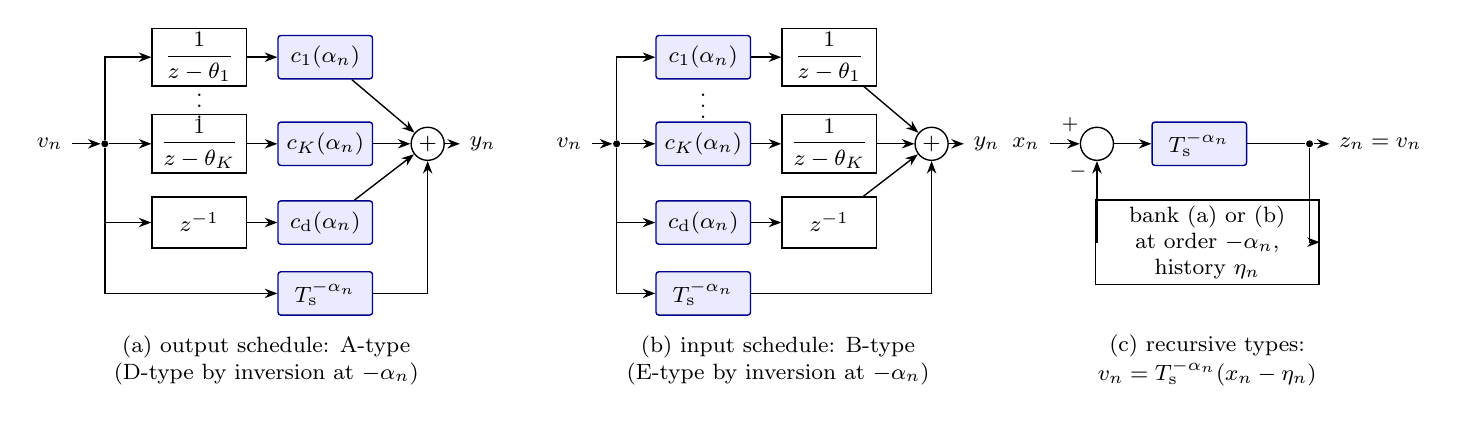
\begin{tikzpicture}[>={Stealth[length=1.6mm]}, font=\footnotesize, line width=0.5pt,
  blk/.style={draw, minimum height=6.5mm, minimum width=12mm, inner sep=1.5pt},
  gain/.style={draw=blue!55!black, fill=blue!8, rounded corners=1pt, minimum height=5.5mm, minimum width=12mm, inner sep=1pt},
  sum/.style={draw, circle, minimum size=4.2mm, inner sep=0pt},
  dot/.style={circle, fill, inner sep=0.9pt}]
\begin{scope}
\node (in) at (0,0) {$v_n$};
\node[dot] (sp) at (0.7,0) {};
\node[blk] (b1) at (1.9,1.1) {$\dfrac{1}{z-\theta_1}$};
\node at (1.9,0.58) {$\vdots$};
\node[blk] (bK) at (1.9,0.0) {$\dfrac{1}{z-\theta_K}$};
\node[blk] (bd) at (1.9,-1.0) {$z^{-1}$};
\node[gain] (c1) at (3.5,1.1) {$c_1(\alpha_n)$};
\node[gain] (cK) at (3.5,0.0) {$c_K(\alpha_n)$};
\node[gain] (cd) at (3.5,-1.0) {$c_{\mathrm d}(\alpha_n)$};
\node[gain] (g0) at (3.5,-1.9) {$\Ts^{-\alpha_n}$};
\node[sum] (S) at (4.8,0) {$+$};
\node (out) at (5.5,0) {$y_n$};
\draw[->] (in) -- (sp); \draw[->] (sp) |- (b1); \draw[->] (sp) -- (bK); \draw[->] (sp) |- (bd); \draw[->] (sp) |- (g0);
\draw[->] (b1) -- (c1); \draw[->] (bK) -- (cK); \draw[->] (bd) -- (cd);
\draw[->] (c1) -- (S); \draw[->] (cK) -- (S); \draw[->] (cd) -- (S); \draw[->] (g0) -| (S); \draw[->] (S) -- (out);
\node[align=center] at (2.75,-2.75) {(a) output schedule: A-type\\(D-type by inversion at $-\alpha_n$)};
\end{scope}
\begin{scope}[xshift=6.6cm]
\node (in) at (0,0) {$v_n$};
\node[dot] (sp) at (0.6,0) {};
\node[gain] (c1) at (1.7,1.1) {$c_1(\alpha_n)$};
\node at (1.7,0.58) {$\vdots$};
\node[gain] (cK) at (1.7,0.0) {$c_K(\alpha_n)$};
\node[gain] (cd) at (1.7,-1.0) {$c_{\mathrm d}(\alpha_n)$};
\node[gain] (g0) at (1.7,-1.9) {$\Ts^{-\alpha_n}$};
\node[blk] (b1) at (3.3,1.1) {$\dfrac{1}{z-\theta_1}$};
\node[blk] (bK) at (3.3,0.0) {$\dfrac{1}{z-\theta_K}$};
\node[blk] (bd) at (3.3,-1.0) {$z^{-1}$};
\node[sum] (S) at (4.6,0) {$+$};
\node (out) at (5.3,0) {$y_n$};
\draw[->] (in) -- (sp); \draw[->] (sp) |- (c1); \draw[->] (sp) -- (cK); \draw[->] (sp) |- (cd); \draw[->] (sp) |- (g0);
\draw[->] (c1) -- (b1); \draw[->] (cK) -- (bK); \draw[->] (cd) -- (bd);
\draw[->] (b1) -- (S); \draw[->] (bK) -- (S); \draw[->] (bd) -- (S); \draw[->] (g0) -| (S); \draw[->] (S) -- (out);
\node[align=center] at (2.65,-2.75) {(b) input schedule: B-type\\(E-type by inversion at $-\alpha_n$)};
\end{scope}
\begin{scope}[xshift=13.0cm]
\node (in) at (-0.6,0) {$x_n$};
\node[sum] (S) at (0.3,0) {};
\node at ($(S)+(-0.34,0.24)$) {\scriptsize $+$};
\node at ($(S)+(-0.24,-0.36)$) {\scriptsize $-$};
\node[gain] (g) at (1.6,0) {$\Ts^{-\alpha_n}$};
\node[dot] (tap) at (3.0,0) {};
\node (out) at (3.9,0) {$z_n=v_n$};
\node[draw, align=center, text width=27mm, minimum height=9mm, inner sep=2pt] (bank) at (1.7,-1.25) {bank (a) or (b) at order $-\alpha_n$, history $\eta_n$};
\draw[->] (in) -- (S); \draw[->] (S) -- (g); \draw[->] (g) -- (tap) -- (out);
\draw[->] (tap) |- (bank.east); \draw[->] (bank.west) -| (S.south);
\node[align=center] at (1.7,-2.75) {(c) recursive types:\\$v_n=\Ts^{-\alpha_n}(x_n-\eta_n)$};
\end{scope}
\end{tikzpicture}}
\caption{Fixed-pole bank. The poles $\theta_k$ and the delay $z^{-1}$ are common to every order; only the shaded weights depend on $\alpha_n$. (a) Order in the output weights. (b) Order in the input weights. (c) Recursive types: the history of bank (a) or (b) at order $-\alpha_n$ is removed and scaled by $1/\gh_0(-\alpha_n)=\Ts^{-\alpha_n}$.}\label{fig:bank}
\end{figure*}

%% =====================================================================
\section{Definition by structure}\label{sec:structure}

\begin{proposition}[Definition by structure]\label{prop:structure}
For every order sequence in $(-1,1)$, every input $v$ and zero initial state, OS gives $y_n=\sum_{r=0}^{n}\gh_r(\alpha_n)v_{n-r}$ and IS gives $y_n=\sum_{r=0}^{n}\gh_r(\alpha_{n-r})v_{n-r}$: the output-scheduled bank is the A-type and the input-scheduled bank the B-type, with the realized weights.
\end{proposition}
\begin{proof}
In OS, $s_k[n]=\sum_{r\ge1}\theta_k^{\,r-1}v_{n-r}$ and $\sd[n]=v_{n-1}$, so $\eta_n=\sum_{r\ge1}\gh_r(\alpha_n)v_{n-r}$. In IS, $s_k[n]=\sum_{r\ge1}\theta_k^{\,r-1}c_k(\alpha_{n-r})v_{n-r}$ and $\sd[n]=\cd(\alpha_{n-1})v_{n-1}$, so $\eta_n=\sum_{r\ge1}\gh_r(\alpha_{n-r})v_{n-r}$.
\end{proof}

No switching term appears, so the accuracy is set by the frozen-order design alone. Let $\eps_R=\sup_a\max_{1\le r<R}|\gh_r(a)/g_r(a)-1|$ over the design range of orders. For $n<R$, in OS,
\begin{equation}
\big|y_n-(\Op{A}{\alpha}v)_n\big|\le\eps_R\textstyle\sum_{r\ge1}|g_r(\alpha_n)|\,|v_{n-r}|,\label{eq:bound}
\end{equation}
and the same with $\alpha_{n-r}$ for IS and the B-type. The bound is relative to the weights: for derivatives, whose weights nearly cancel, relative output errors for smooth inputs can exceed $\eps_R$.

\begin{proposition}[Recursive types by inversion]\label{prop:inverse}
Run the OS (IS) bank at the orders $-\alpha$ with history $\eta_n$. The recursion $v_n=\Ts^{-\alpha_n}(x_n-\eta_n)$, $z_n=v_n$, gives $z=\hat W_{\mathrm A}(-\alpha)^{-1}x$ ($\hat W_{\mathrm B}(-\alpha)^{-1}x$): the D-type (E-type) with realized weights, with the duality~\eqref{eq:duality} exact in exact arithmetic, at $O(K)$ per sample.
\end{proposition}
\begin{proof}
By Proposition~\ref{prop:structure}, row $n$ of $\hat W_{\mathrm A}(-\alpha)v=x$ is $\Ts^{\alpha_n}v_n+\eta_n=x_n$, solved forward since $\Ts^{\alpha_n}\neq0$.
\end{proof}

Because every row of the A-type error matrix and every column of the B-type error matrix holds a single order, the weight errors also bound the realized operators as a whole. Let $\|\cdot\|_p$ be the induced $\ell^p$ norm of an $N\times N$ matrix and $|M|$ its entrywise modulus.

\begin{theorem}[Operator-norm bounds]\label{thm:opnorm}
Let $\mathcal S\subset(-1,1)$, $N\le R$, $e_r(a)=\gh_r(a)-g_r(a)$, $\rho_{\mathrm{row}}=\sup_{a\in\mathcal S}\sum_{r=1}^{N-1}|e_r(a)|$ and $\rho_{\mathrm{col}}=\sum_{r=1}^{N-1}\sup_{a\in\mathcal S}|e_r(a)|$. For every order sequence in $\mathcal S$, with $E_{\mathrm T}=\hat W_{\mathrm T}-W_{\mathrm T}$:
\begin{enumerate}
\item[(a)] $\|E_{\mathrm A}\|_\infty\le\rho_{\mathrm{row}}$, $\|E_{\mathrm A}\|_1\le\rho_{\mathrm{col}}$, $\|E_{\mathrm B}\|_1\le\rho_{\mathrm{row}}$, $\|E_{\mathrm B}\|_\infty\le\rho_{\mathrm{col}}$; each bound is attained for finite $\mathcal S$.
\item[(b)] $\|E_{\mathrm T}\|_p\le\eps_R\|\,|W_{\mathrm T}|\,\|_p$ for $1\le p\le\infty$, $\mathrm T\in\{\mathrm A,\mathrm B\}$; for $p\in\{1,\infty\}$ the relative operator error, i.e.\ the worst-case relative output error, never exceeds $\eps_R$.
\item[(c)] For $(\mathrm T,\mathrm F)\in\{(\mathrm D,\mathrm A),(\mathrm E,\mathrm B)\}$, let $E^-_{\mathrm F}$ be the error of $\hat W_{\mathrm F}(-\alpha)$ and $q=\|W_{\mathrm T}\|_p\|E^-_{\mathrm F}\|_p<1$. Then $\|E_{\mathrm T}\|_p\le\frac{q}{1-q}\|W_{\mathrm T}\|_p$, and the same holds with the realized $\hat W_{\mathrm T}$ in place of $W_{\mathrm T}$. If all orders are negative and $\gh_1(-\alpha_n)<0$ for all $n$, then $\hat W_{\mathrm T}\ge0$ entrywise and $\|\hat W_{\mathrm T}\|_\infty$ is the peak of the realized step response: one step response of the bank ($O(NK)$) certifies the error a posteriori.
\end{enumerate}
\end{theorem}

The proof is in \proofref{app:opnorm}. By (b), $q\le\eps_R\kappa_p$ with $\kappa_p=\|W_{\mathrm F}\|_p\|W_{\mathrm F}^{-1}\|_p$; for a constant order $a$, $\kappa_\infty=(2-w_{N-1}(a-1))w_{N-1}(-a-1)\approx2N^a/\Gamma(1+a)$, 71 for $a=0.5$, $N=1000$. For recursive integrals this amplification is real, so a guaranteed design uses $\eps/\kappa_\infty$.

The fixed-pole structure is also necessary in the following sense.

\begin{theorem}[Necessity]\label{thm:necessity}
Let $\Sigma_i=(F_i,b_i,c_i^{\top},d_i)$, $i=1,2$, be minimal realizations of dimension $S$ of two frozen-order operators, run as $\Sigma_1$ for $n<m$ and $\Sigma_2$ for $n\ge m$, $m\ge S+1$, with the state mapped as $x[m]\leftarrow\Phi x[m]$.
(a) For every input, the output for $n\ge m$ is the response of $\Sigma_2$ to the whole input (A-type behaviour) iff $F_2=\Phi F_1\Phi^{-1}$ and $b_2=\Phi b_1$.
(b) It is the response of $\Sigma_1$ to the inputs before $m$ plus that of $\Sigma_2$ to the inputs from $m$ on (B-type behaviour) iff $F_2=\Phi F_1\Phi^{-1}$ and $c_2^{\top}=c_1^{\top}\Phi^{-1}$.
\end{theorem}

The proof is in \proofref{app:necessity}; the same statement holds in continuous time.

\begin{corollary}\label{cor:moving}
If the poles of a frozen-order realization depend on the order, as in the Oustaloup family~\cite{oustaloup2000}, no state map (in particular not the hot swap $\Phi=I$) realizes the A- or B-type at a switch. The fixed-pole bank satisfies (a) with $\Phi=I$ in OS and (b) with $\Phi=I$ in IS.
\end{corollary}

Least-squares maps fitted to an input ensemble can make the definitional error small in floating point, but they are dense, specific to each pair of orders, depend on the input statistics, and lose 3 to 9 orders of magnitude of accuracy in 24-bit arithmetic (Supplementary Material).

%% =====================================================================
\section{Completely monotone kernel families}\label{sec:cm}

The construction used two properties of the GL weights: for each order they are a superposition of geometric sequences with a density of one sign, smooth on a logarithmic scale. A family of causal kernels $\{k_a\}_{a\in\mathcal A}$ is a \emph{completely monotone (CM) family} if $k_a(0)\neq0$ and $k_a(r)=\sigma_a\int_0^\infty e^{-(r-1)u}m_a(u)\,\mathrm du$ for $r\ge1$, with $\sigma_a\in\mathbb R$ and $m_a\ge0$; by Hausdorff's theorem these are the completely monotone sequences~\cite{widder1941}. Its A- and B-types are~\eqref{eq:A},~\eqref{eq:B} with $k_a(r)$ in place of $g_r(a)$, and its D- and E-types follow from~\eqref{eq:duality}. The bank is built as above, with residues $c_k(a)=\sigma_ahu_km_a(u_k)$.

\begin{theorem}[CM families]\label{thm:cm}
(a) Propositions~\ref{prop:structure} and~\ref{prop:inverse} and Theorems~\ref{thm:opnorm} and~\ref{thm:necessity} hold for every CM family; the parameter $a$ need not be an order, and all residues have the sign of $\sigma_a$.
(b) Assume: (H1) $f_{a,r}(x)=e^xm_a(e^x)e^{-(r-1)e^x}$ is analytic in $|\mathrm{Im}\,x|<d<\pi/2$ with $L_d=\sup_{a,r,|y|<d}\int|f_{a,r}(x+\mathrm iy)|\mathrm dx/\int f_{a,r}<\infty$; (H2) $c_-u^{\beta_a-1}\le m_a(u)\le c_+u^{\beta_a-1}$ on $(0,u_*]$, $\beta_a\in[\beta_-,\beta_+]$; (H3) $m_a(u)\le C_\infty e^{-\gamma u}$ on $[u_*,\infty)$. Let $\vartheta=\min_{\beta_-\le\beta\le\beta_+}\int_0^{u_*}t^{\beta-1}e^{-t}\mathrm dt$, $C_{\mathrm{lo}}=c_+/(c_-\beta_-\vartheta)$ and $C_{\mathrm{hi}}=C_\infty/((1+\gamma)c_-\vartheta)$. Then, for $\ulo\le u_*$, $\uhi\ge\max(u_*,1,\beta_+\ln2)$ and $1\le r<R$,
\begin{equation}
\begin{aligned}
\Big|\frac{\hat k_a(r)}{k_a(r)}-1\Big|\le{}&\frac{2L_d}{e^{2\pi d/h}-1}+C_{\mathrm{lo}}\big((R-1)\ulo\big)^{1+\beta_a}\\
&+C_{\mathrm{hi}}\,e^{-(1+\gamma)\uhi}.
\end{aligned}\label{eq:cmerr}
\end{equation}
(c) For $0<\eps\le\min(1,4C_{\mathrm{lo}})$, $h=2\pi d/\ln(1+4L_d/\eps)$, $\ulo=\min(u_*,(\eps/4C_{\mathrm{lo}})^{1/(1+\beta_-)}/(R-1))$, $\uhi=\max(u_*,1,\beta_+\ln2,\ln(4C_{\mathrm{hi}}/\eps)/(1+\gamma))$ and $K=\lceil\ln(\uhi/\ulo)/h\rceil+1$, the relative weight error is at most $\eps$ for all $a$ and $1\le r<R$, and $K=O(\ln(1/\eps)\ln(R/\eps))$ uniformly in $a$.
\end{theorem}

\begin{lemma}[GL constants]\label{lem:glconst}
For $|a|\le\bar a<1$, the GL family satisfies (H1)--(H3) for every $d<\pi/2$ with $\beta_a=1+a$, $\gamma=1-\bar a$, $u_*=1$, $c_-=(1-e^{-1})e^{-2}$, $c_+=C_\infty=(1-e^{-1})^{-1}$ and $L_d\le(2/(1-e^{-2}))^{\bar a}(\cos d)^{-(1+\bar a)}$.
\end{lemma}

The proofs are in \proofref{app:cm}. With $h\approx\pi^2/\ln(1/\eps)$, part (c) gives $K\approx\ln(1/\eps)\ln(R/\eps)/\pi^2$ to leading order. Examples are time-varying distributed orders, whose bank has the same poles and averaged residues (A- and B-types still at $O(K)$), and fixed tempering $e^{-\lambda r}g_r(a)$~\cite{sabzikar2015}, realized exactly by the poles $e^{-\lambda}\theta_k$; a tempering parameter that varies in time moves the poles and falls under Theorem~\ref{thm:necessity}. In continuous time Bernstein's theorem plays the role of Hausdorff's~\cite{widder1941,mainardi2015}.

%% =====================================================================
\section{Design rule and inverse stability}\label{sec:design}

The rule chooses $h$, $\ulo$, $\uhi$ and $K$ from $\eps$, the memory $R$ (samples) and an order range, without fitted constants. With the tail closure the realized weights are the infinite trapezoidal rule applied to~\eqref{eq:betax} apart from two tail residuals, so the error has three terms. The quadrature term is the first alias of the strip-analytic integrand (Poisson summation~\cite{trefethen2014}); for large $r$, Stirling's formula gives
\begin{equation}
E_q^{\infty}(a,h)=2\sqrt{2\pi}\,(2\pi/h)^{a+1/2}e^{-\pi^2/h}/\Gamma(1+a),\label{eq:Eq}
\end{equation}
and small lags are evaluated directly. The lower-tail residual grows with the lag, $E_{\mathrm{lo}}=(r-1)\ulo^{2+a}H_h(1+a,2+a)/\Beta(r-a,1+a)$ at $r=R-1$ with $H_h(p,q)=G_h(p)-G_h(q)$, $G_h(p)=h/(e^{ph}-1)$, which ties $\ulo$ to the memory; the upper-tail residual appears first at $r=2$. The tolerance is split $\eps/2$, $\eps/4$, $\eps/4$: $h$ from the quadrature term (a one-dimensional root), $\ulo$ in closed form, $\uhi$ by a monotone root, and $K=\lceil\ln(\uhi/\ulo)/h\rceil+1$.

The recursive types run $1/\Hh$, whose dynamics matrix has the characteristic polynomial $z\prod_k(z-\theta_k)\Hh(z)/\gh_0$ in both schedules.

\begin{proposition}[Inverse stability]\label{prop:stability}
Let $\Hh(z)=g_0+\cd/z+\sum_kc_k/(z-\theta_k)$, $g_0>0$, distinct $\theta_k\in(0,1)$. (i) If all $c_k>0$ and $\cd\ge0$ (integral bank), $1/\Hh$ is stable iff $\Hh(-1)>0$. (ii) If all $c_k<0$ (derivative bank), $1/\Hh$ is stable iff $\Hh(1)>0$ and either $\cd\le0$ or $\Hh(-1)>0$. (iii) If $|\gh_r/g_r-1|\le1/3$ for $r=1,2$, then $\Hh(-1)>0$.
\end{proposition}

The proof is in \proofref{app:stability}. So an integral bank of the rule always has a stable inverse, and a derivative bank has one iff its realized DC gain $\Hh(1)=\sum_r\gh_r$ is positive. The exact GL derivative has $\sum_rg_r=0$; the finite memory adds about $S_a\Ts^{-a}\ulo^{a}/(a(1+a))$, which for large orders can be smaller than the quadrature error. A DC floor raises the delay residue to $\Hh(1)\ge0.01\,S_a\Ts^{-a}\ulo^a/(a(1+a))$, changing only $\gh_1$, and makes every inverse stable. The signs of $\Hh(\pm1)$ are computed to full precision, unlike the dominant pole, which lies within $10^{-9}$ of $z=1$.

%% =====================================================================
\section{Numerical results}\label{sec:results}

Unless stated otherwise, $\Ts=1$\,ms; references are the literal definitions~\eqref{eq:A}--\eqref{eq:E} evaluated in $O(N^2)$. The \emph{definitional error} is the distance of a switched realization from its \emph{own} A-, B-, D- or E-type built from the same frozen-order systems. Baselines are Oustaloup approximations~\cite{oustaloup2000} with $S=2N+1$ states in parallel and cascade form, discretized by zero-order hold and hot-swapped.

\emph{Definition consistency.} A bank with 32 modes was compared with the GL types over 7 order profiles and 3 inputs: OS against the A-type and IS against the B-type gave total errors of $1.9\times10^{-6}$ to $2.0\times10^{-3}$. The definitional errors (Table~\ref{tab:e1b}) are zero to rounding for the bank, as Proposition~\ref{prop:structure} predicts, and reach $3\times10^3$ for the hot-swapped cascade. One bank ($K=41$) ran all four types within $6.9\times10^{-5}$ of the literal definitions, with the duality~\eqref{eq:duality} exact to $2\times10^{-14}$.

\begin{table}[t]
\caption{Definitional error under piecewise-constant orders (discrete time; Oustaloup with $S=31$)}\label{tab:e1b}
\centering\footnotesize\setlength{\tabcolsep}{3pt}
\begin{tabular}{@{}lcc@{}}
\toprule
Realization & vs own A-type & vs own B-type\\
\midrule
bank, output schedule & 0 (exact) & = A--B gap\\
bank, input schedule & = A--B gap & $\le10^{-14}$\\
Oustaloup parallel, hot swap & $4\times10^{-6}$--$0.13$ & $7\times10^{-3}$--$1.0$\\
Oustaloup cascade, hot swap & $7\times10^{-3}$--$3\times10^{3}$ & $0.03$--$4.8\times10^{2}$\\
\bottomrule
\end{tabular}
\end{table}

\emph{Design rule on a sealed holdout.} With each error term isolated, the ratio of measured to predicted error was 0.49--1.05 in discrete and 0.99--1.01 in continuous time. We then drew 400 random specifications ($\eps\in[10^{-5},10^{-2}]$, $R\in[10^2,10^5]$ or 0.5 to 6 decades, random order ranges in $[-0.95,0.95]$), recorded their SHA-256 digest before evaluation, and evaluated them once\ifsp\else{} (Fig.~\ref{fig:rule})\fi: all 400 were met (one-sided 95\,\% Clopper--Pearson bound 98.5\,\% per domain~\cite{clopper1934}), at a median 0.41--0.50 of $\eps$, with $K$ at most three modes above the smallest sufficient size. Each decade of memory adds about three modes and each decade of accuracy seven to ten ($K=29$ for $\eps=10^{-4}$, $R=10^3$). Over 35 designs the fit $K\approx0.57+1.06\ln(1/\eps)+0.53\ln R+0.106\ln(1/\eps)\ln(R/\eps)$ reproduces every $K$ within 0.7 modes; Theorem~\ref{thm:cm} predicts $1/\pi^2=0.101$ for the product term. With the constants of Lemma~\ref{lem:glconst}, part (c) of Theorem~\ref{thm:cm} gives guaranteed banks 1.4--1.6 times the size of the rule, with errors 13--17 times below $\eps$. With the DC floor the inverse was stable in all 200 discrete-time holdout designs (101 of 200 without it).

\ifsp\else\input{\partsdir fig_rule}\fi
\emph{Operator norms.} For $N=1000$ and eleven order sequences, including two adversarial ones, the dense realized and literal operators gave Table~\ref{tab:opnorm}. No A- or B-type norm exceeded its bound, the bounds of part (a) were attained to four digits, and the relative operator error was at most $0.45\,\eps_R$. For the recursive types the relative error reached 22 times $\eps_R$, as the conditioning predicts, and the certificate of part (c) held.

\begin{table}[t]
\caption{Theorem~\ref{thm:opnorm} on dense operators ($N=1000$, eleven order sequences): measured over bounded quantities}\label{tab:opnorm}
\centering\footnotesize\setlength{\tabcolsep}{3pt}
\begin{tabular}{@{}llcc@{}}
\toprule
Types & Quantity & $K=22$ & $K=49$\\
\midrule
A, B & $\|E\|_p/$bound (a), $p=1,\infty$ & 0.28--1.00 & 0.45--1.00\\
A, B & $(\|E\|_p/\|W\|_p)/\eps_R$ & 0.04--0.39 & 0.03--0.45\\
D, E integrals & $\|E\|_\infty/$bound (c) & 0.23--0.31 & 0.006--0.23\\
D, E & $\max(\|E\|_\infty/\|W\|_\infty)/\eps_R$ & 22 & 17\\
\bottomrule
\end{tabular}
\end{table}

\emph{Cost against accuracy.} Fig.~\ref{fig:pareto} compares four realizations of the A-type over 39 order levels ($N=1000$): the fixed-pole bank of the rule; fixed poles with residues fitted per level by a linear program, without and with the sign and DC constraints of Proposition~\ref{prop:stability}; moving poles (a rule-designed grid per level, hot-swapped); and truncated GL convolution. Moving poles reach a constant-order accuracy with two thirds of the states, but stay at 0.72--1.1 (A) and 0.17--0.23 (B) under switching for every $K$, as Theorem~\ref{thm:necessity} predicts. Integral orders need the whole memory: truncation leaves 0.41 at $L=512$. Fitted residues save 40--50\,\% of the poles unconstrained, but then lose the stability certificate at up to 11 of 19 derivative levels; with the constraints the saving is 20--30\,\%. The rule thus trades a fifth to a quarter of the states for a closed-form, validated design that keeps the residue signs.

\begin{figure*}[t]
\centering
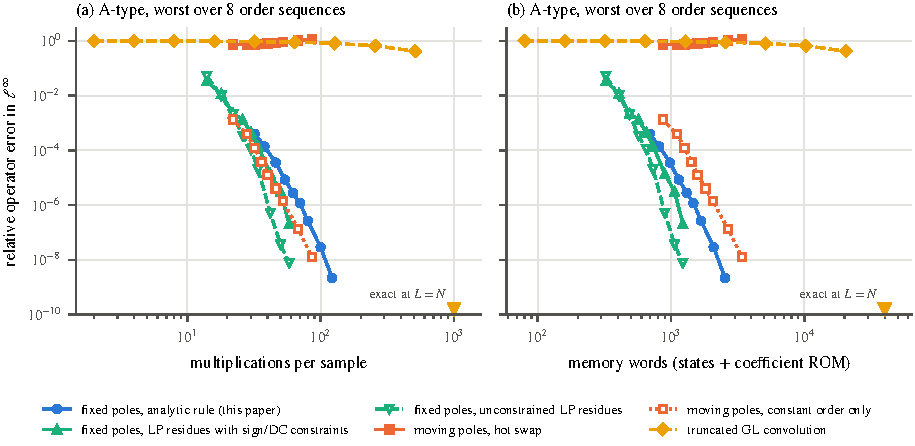
\includegraphics[width=0.86\textwidth]{fig_pareto.pdf}
\caption{Accuracy against cost for the A-type ($N=1000$, 39 order levels). Solid: worst relative operator error over eight variable-order sequences; dotted: moving poles at constant order only.}\label{fig:pareto}
\end{figure*}

%% =====================================================================
\section{Order tracking}\label{sec:track}

Consider a fractional element, such as an ultracapacitor or a viscoelastic material, excited by a known input $x$ while its memory exponent drifts. The task is to track the order from
\begin{equation}
y_n=\big(\Op{T}{\alpha}x\big)_n+v_n,\qquad v_n\sim\mathcal N(0,\sigma^2),\qquad \mathrm T\in\{\mathrm A,\mathrm B\},\label{eq:trackmodel}
\end{equation}
with a random walk $\alpha_{n+1}=\alpha_n+w_n$, $w_n\sim\mathcal N(0,q)$. Unscented fractional-order Kalman filters (UFOKF) keep the order in the filter state and evaluate the GL memory directly~\cite{sierociuk2016cssp}. The bank provides the measurement model and its derivative at $O(K)$ cost for either type, and its structure decides which estimator is natural.

\emph{A-type.} With the order in the output weights, the states of OS are driven by the known input alone, so $y_n=\varphi_n(\alpha_n)+v_n$ with $\varphi_n(a)=\Ts^{-a}x_n+\cd(a)\sd[n]+c(a)^{\top}s_n$: a memoryless measurement of the current order whose regressors are shared by all orders. An extended Kalman filter (EKF) needs $\varphi_n$ and $\varphi_n'$, at $O(K)$; the exact likelihood of $G$ order hypotheses costs $O(GK)$, so a grid (point-mass) Bayes filter becomes affordable.

\emph{B-type.} With the order in the input weights, the state of IS carries the order history, and an EKF on $(s,\sd,\alpha)$ of dimension $K+2$ costs $O(K^2)$; in the literal GL form the filter would have to carry the whole order history.

\emph{Bayesian Cram\'er--Rao bound.} With Gaussian noise of known variance, the Fisher information of the order path given the path is $G^{\top}G/\sigma^2$, where $G$ is the Jacobian of the noise-free output. It is diagonal for the A-type, $G_{nn}=h_n=\sum_{r\ge1}w_r'(\alpha_n)x_{n-r}$, and strictly lower triangular for the B-type, $G_{nm}=w'_{n-m}(\alpha_m)x_m$ for $m<n$, where $w_r'=\partial w_r/\partial a$ follows by differentiating the recursion~\eqref{eq:glw}. Its expectation over the prior of the path, plus the information of the random walk, is the Bayesian (Van Trees) information, whose inverse bounds the mean-square error of every estimator; restricted to the data up to $n$ it gives the filtering bound of causal estimators~\cite{tichavsky1998}. For the A-type the information is diagonal and $J_n=(q+J_{n-1}^{-1})^{-1}+\mathbb E[h_n^2]/\sigma^2$. For the B-type in sample units, $\gh_0=1$ for every order, so $\alpha_n$ does not enter $y_n$; its information arrives only later, through the memory. The causal estimate of the present B-type order is therefore essentially a prediction from the past, and the smoothing bound (all data) can lie far below the filtering bound. We condition on the known input, average the information over prior paths by Monte Carlo, and obtain both bounds from a Kalman recursion on the growing path ($O(n^3)$, off line).

\emph{Experiments.} In sample units ($n=2000$), with a known AR(1) input of pole 0.98, data from the literal GL definitions, white noise at 20, 40 and 60\,dB and 50 Monte Carlo runs, one rule-designed bank ($\eps=10^{-5}$, $|\alpha|\le0.95$, $K=40$, coefficients interpolated by cubic splines) served all estimators. In the first scenario the order is constant at 0.3, ramps to 0.7, jumps to 0.2 and then oscillates; the EKFs inflate the order variance when the normalized innovation exceeds 16, which detects jumps, and the grid filter (381 orders) mixes its random walk ($q=10^{-5}$) with a uniform switch. Every estimator was also run on data of the other type. In the second scenario the orders are drawn from the random-walk prior itself ($q=10^{-5}$, $\alpha_0\sim\mathcal N(0.3,0.01)$), and the estimators, tuned to it without jump gating, are compared with the bounds.

\begin{table}[t]
\caption{Order tracking with a ramp and a jump: median RMSE of the order over $0.2\le t<4$\,s (50 runs). ``Wrong'': data of the other type. Costs are multiplications per sample ($K=40$, $G=381$, $n=2000$)}\label{tab:track}
\centering\tabfont\setlength{\tabcolsep}{2.4pt}
\begin{tabular}{@{}llccc@{}}
\toprule
Estimator (cost) & Data & 20\,dB & 40\,dB & 60\,dB\\
\midrule
A-type grid filter ($\approx16\,000$) & A & 0.018 & 0.0040 & 0.0013\\
 & B, wrong & 0.029 & 0.059 & 0.140\\
A-type EKF ($\approx3(K+2)$/iteration) & A & 0.026 & 0.0083 & 0.017\\
 & B, wrong & 0.037 & 0.099 & 0.213\\
B-type EKF ($\approx4(K+2)^2$) & B & 0.027 & 0.015 & 0.012\\
 & A, wrong & 0.032 & 0.054 & 0.238\\
\midrule
\multicolumn{5}{@{}l}{\emph{UFOKF-type unscented filters on the GL sum (our implementation)}}\\
A-type, memory 100 ($\approx600$) & A & 0.036 & 0.138 & 0.244\\
A-type, full memory ($\approx3n$) & A & 0.027 & 0.016 & 0.039\\
B-type, window 5 ($\approx n$) & B & 0.028 & 0.014 & 0.012\\
\bottomrule
\end{tabular}
\end{table}

\ifsp\else\input{\partsdir fig_tracking}\fi
\emph{Results with a jump} (Table~\ref{tab:track}\ifsp\else, Fig.~\ref{fig:tracking}\fi). With the matched type the error decreases with the SNR, to $1.3\times10^{-3}$ for the A-type grid filter and $1.2\times10^{-2}$ for the B-type EKF at 60\,dB. With the wrong type it \emph{increases} with the SNR, to 0.14--0.24 at 60\,dB: a wrong definition biases the estimate, and more data do not remove the bias. While the order is constant the two definitions coincide and both filters are accurate; the bias appears as soon as the order varies. The A-type EKF has a heavy tail at high SNR (90th percentile 0.11--0.15), because the likelihood of one sample has several maxima at the jump; the grid filter avoids this. The A-type EKF on the bank reproduced the same EKF on the literal GL weights to $9\times10^{-6}$, at about $3(K+2)$ instead of $3n$ multiplications per iteration, and the full-memory UFOKF-type filter and the same filter on the bank agreed to $10^{-4}$ in 144 of 150 runs. A truncated GL memory biases the estimate (0.24 at 60\,dB with 100 lags). For the B-type, the windowed unscented filter matched the bank's EKF, but it keeps and updates the whole input history, $O(n)$ per sample, whereas the bank's state has $K+2$ entries.

\begin{table}[t]
\caption{Random-walk orders drawn from the prior: RMSE of the order over runs and over $0.2\le t<4$\,s, and the Bayesian CRB conditioned on the known input (50 runs; ratio to the filtering bound in brackets)}\label{tab:crb}
\centering\tabfont\setlength{\tabcolsep}{3pt}
\begin{tabular}{@{}llccc@{}}
\toprule
Data & & 20\,dB & 40\,dB & 60\,dB\\
\midrule
A & grid filter & 0.0128 [1.14] & 0.0046 [1.30] & 0.0016 [2.14]\\
 & EKF & 0.0128 [1.15] & 0.0046 [1.30] & 0.0014 [1.82]\\
 & filtering BCRB & 0.0112 & 0.0035 & 0.00074\\
 & smoothing BCRB & 0.0079 & 0.0027 & 0.00067\\
\midrule
B & augmented EKF & 0.0134 [1.06] & 0.0056 [1.01] & 0.0035 [1.00]\\
 & filtering BCRB & 0.0127 & 0.0055 & 0.0035\\
 & smoothing BCRB & 0.0083 & 0.0032 & 0.0011\\
\bottomrule
\end{tabular}
\end{table}

\begin{figure}[t]
\centering
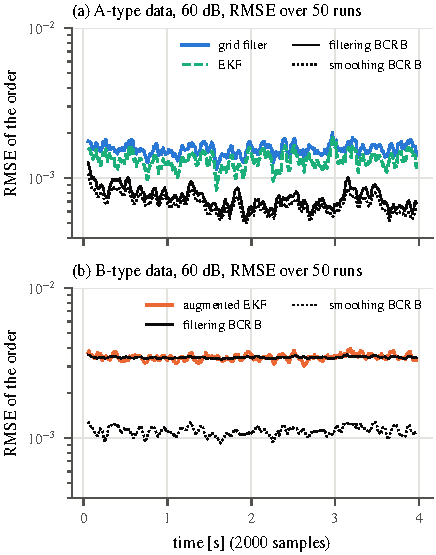
\includegraphics[width=\colfigwidth]{fig_crb.pdf}
\caption{Random-walk orders at 60\,dB: RMSE of the order over 50 runs (running mean over 28 samples) and the Bayesian CRB conditioned on the input, for causal estimators (filtering) and with all data (smoothing).}\label{fig:crb}
\end{figure}

\emph{Results against the bound} (Table~\ref{tab:crb}, Fig.~\ref{fig:crb}). The B-type EKF attains the filtering bound: its RMSE is 1.06, 1.01 and 1.00 times the bound at 20, 40 and 60\,dB. The A-type filters are within a factor of 1.15 at 20\,dB and 1.3 at 40\,dB. At 60\,dB the grid filter is limited by its spacing (0.005, i.e.\ $1.4\times10^{-3}$ RMS), and the EKF stays 1.8 times above the bound. The EKF on the bank reproduces the EKF on the literal GL weights (to $9\times10^{-6}$ in the first scenario), so the gap is not due to the bank; a Bayesian bound need not be attainable. The two types differ structurally. For the A-type the smoothing bound is close to the filtering bound, because each sample measures the present order. For the B-type it is three times lower at 60\,dB: the present order is observed only through later samples, so a fixed-lag smoother could gain up to a factor of three, while no causal estimator can.

%% =====================================================================
\section{Measured data: a lithium-ion cell}\label{sec:battery}

Fractional elements are common in battery models~\cite{zou2018review}, and variable-order versions let the order depend on the state of charge~\cite{lu2018energies,wang2022symmetry,mao2023est}. Once the order moves, a model identified with one definition and executed by a realization of the other is a different model. We tested how much this matters on public measurements of a Panasonic 18650PF cell~\cite{kollmeyer2018data}: four drive cycles (UDDS, LA92, US06, HWFET) at each of five chamber temperatures from 25 to $-20\,^\circ$C, and two warming runs of four mixed cycles each (10 to 24--27\,$^\circ$C and $-20$ to 12--17\,$^\circ$C).

\emph{Model.} With the terminal voltage $v$, the current $i$ (positive for charge), the state of charge $z$ from coulomb counting and the open-circuit voltage $U$ of the C/20 test at 25\,$^\circ$C,
\begin{equation}
\begin{aligned}
v_n-U(z_n)={}&c(z_n)+R_0(z_n)\,i_n+R_1(z_n)\,(\psi_\tau i)_n\\
&+\kappa(z_n)\big(\Op{T}{-\beta(z)}i\big)_n,\qquad \mathrm T\in\{\mathrm A,\mathrm B\},
\end{aligned}\label{eq:battery}
\end{equation}
at $\Ts=1$\,s, where $\psi_\tau$ is a unit-gain first-order lag, the gains are piecewise linear in $z$ (knots 0.1 apart), and the order is piecewise linear in $z$ on six knots, so it changes at every sample. In the A-type the present order weights the whole past current; in the B-type each current sample keeps the order of the moment it flowed. Baselines are a constant order (A $=$ B) and one or two lags instead of the fractional term (1RC, 2RC). For fixed $\tau$ and order knots the gains follow from least squares; $\tau$ (1 to 5000\,s) and the knots (0.02 to 0.95) were found by coordinate search. One rule-designed bank ($\eps=10^{-4}$, $R=25\,000$, $K=29$) served all orders and both types; the A-type columns of all 94 grid orders come from one state, and a candidate order path costs $O(nK)$ for either type.

\emph{Protocol.} In each group, every model was fitted jointly to three cycles and simulated the fourth from its current alone, with every parameter, the order included, read from the $z$ of the held-out record. Fits to a single cycle did not transfer (RC+FO: 12\,mV in sample, 92--101\,mV on other cycles, over 84 runs): the slow terms are nearly collinear with $z$, the integral of the current.

\begin{table}[t]
\caption{Battery data: RMSE (mV) of the simulated voltage on the held-out cycle, mean over four folds. The last two columns run the fitted VO models with the operator of the other type. Bold: lowest of the row}\label{tab:battery}
\centering\tabfont\setlength{\tabcolsep}{2.2pt}
\begin{tabular}{@{}lccccccc@{}}
\toprule
 & & & \multicolumn{3}{c}{RC + fractional} & \multicolumn{2}{c}{other type}\\
\cmidrule(lr){4-6}\cmidrule(l){7-8}
Group & 1RC & 2RC & const. & VO-A & VO-B & A as B & B as A\\
\midrule
$25\,^\circ$C & 20.2 & 18.6 & 16.3 & 15.8 & \textbf{14.7} & 94 & 46\\
$10\,^\circ$C & 27.2 & 27.0 & \textbf{25.6} & 37.7 & 26.7 & 44 & 98\\
$0\,^\circ$C & 36.1 & \textbf{35.0} & 36.2 & 36.8 & 36.3 & 49 & 92\\
$-10\,^\circ$C & \textbf{60.6} & 62.7 & 66.7 & 66.7 & 66.9 & 104 & 328\\
$-20\,^\circ$C & \textbf{111.1} & 116.4 & 122.3 & 122.8 & 128.5 & 239 & 1295\\
$10\,^\circ$C, warming & 14.7 & \textbf{13.5} & 15.1 & 14.9 & 14.6 & 23 & 80\\
$-20\,^\circ$C, warming & 34.4 & \textbf{33.1} & 36.8 & 38.1 & 40.4 & 94 & 109\\
\bottomrule
\end{tabular}
\end{table}

\begin{figure*}[t]
\centering
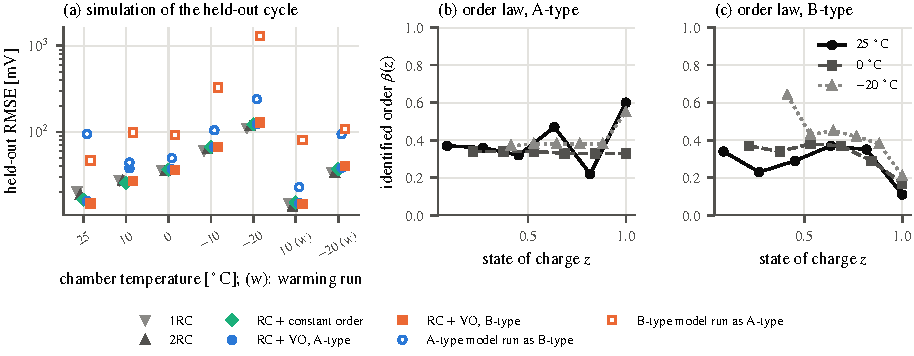
\includegraphics[width=0.9\textwidth]{fig_battery.pdf}
\caption{Battery data. (a) Held-out RMSE (Table~\ref{tab:battery}); hollow markers: fitted VO models run with the operator of the other type. (b, c) Order laws $\beta(z)$ fitted to all four cycles of a temperature with the A- and B-type operators.}\label{fig:battery}
\end{figure*}

\emph{Results.} Run with the A-type operator, the B-type models were worse in all 28 folds, by a median factor of 4.4 (at least 1.06); run with the B-type operator, the A-type models were worse in 23 of 28 folds, by a median factor of 2.1 (Table~\ref{tab:battery}, Fig.~\ref{fig:battery}a). The fitted order laws themselves depend on the definition (Fig.~\ref{fig:battery}b, c): at the five constant temperatures the B-type order drops at the start of the discharge, to 0.11--0.21 at $z=1$ against 0.23--0.64 below, whereas the A-type laws stay within 0.33--0.43 away from $z=1$ (0.22--0.47 at 25\,$^\circ$C) and lie above the B-type ones at $z=1$. An order law reported for a VO battery model is therefore meaningful only with its definition. A varying order helped only at 25\,$^\circ$C, where the B-type model had the lowest held-out error (14.7\,mV against 16.3 for a constant order and 18.6 for 2RC; best in three of four folds). At 0\,$^\circ$C and below, and in both warming runs, an RC model was best, and at 0\,$^\circ$C and below every model erred by 35--128.5\,mV. Linearized at the states of charge of the impedance sweeps in the same data set, every model's impedance magnitude between 1.4\,mHz and 0.1\,Hz was about 0.9 of the measured one at 25 and 10\,$^\circ$C, 0.7 at 0\,$^\circ$C and 0.4 at $-20\,^\circ$C: the drive cycles see a much lower impedance than a small-signal sweep, consistent with a current-dependent charge-transfer resistance and self-heating, which no model linear in the current contains.

\ifsp\else\input{\partsdir tab_battreal}\fi
\emph{Other realizations.} With the same gains and order laws (\ifsp table in the Supplementary Material\else Table~\ref{tab:battreal}\fi), the bank reproduced the literal GL sum to $3.2\times10^{-6}$ at a fixed cost, where the GL sum costs $O(n)$ per sample. Truncating the memory multiplied the error by 6 to 11: the cell remembers its current far beyond 600\,s. Moving poles (one rule-designed bank per order level of a 0.01 grid, hot-swapped) did almost as well as the bank here, because the order laws are smooth and the level changed only between neighbouring grid values; the fractional term deviated from its definition by up to 10\,\%. A moving-pole realization fails at large order steps (Sect.~\ref{sec:results}), not at small ones. On these data the definition and the memory length decide the error; the pole structure matters little. The experiment does not show that a variable order improves battery models in general.

%% =====================================================================
\section{Fixed-point realization and further applications}\label{sec:hw}

\ifsp
A time-multiplexed Verilog core realizes all four types, with order and type as inputs at every sample; an order change is a ROM address. An exact rational test of the signs of $\Hh_q(\pm1)$ of every quantized ROM row, with a quantization-aware DC floor, keeps all inverses stable. On a Zynq-7020 the A/B and A/B/D/E configurations (36 and 48 signal bits) close at 44.3 and 39.3\,MHz with 11 and 15 DSP slices, i.e.\ about 0.3 million samples per second, and on a PYNQ-Z1 board both were bit-exact on all test vectors, including a $2^{24}$-sample D-type run at the worst quantized row. The same bank also streams multifractional Brownian motion of both types~\cite{wang2023mmfbm}. Details are in the Supplementary Material.

\else
In sample units ($\Ts=1$) the inversion of Proposition~\ref{prop:inverse} needs no divider, and the physical gain $\Ts^{-\alpha_n}$ is applied once per sample. A time-multiplexed Verilog core realizes all four types with order and type as inputs at every sample: an order change is a ROM address, with no reload and no extra cycle. With an exact rational test of the signs of $\Hh_q(\pm1)$ for every quantized ROM row, 64 (A/B) and 51 (A/B/D/E) of 512 derivative rows had unstable inverses with the floating-point DC floor alone; a quantization-aware floor, which raises the delay mantissa in LSB steps, brings both to zero. The smallest configurations meeting $0.1\eps$ on a stress set use 36/49/16 (A/B) and 48/61/25 (A/B/D/E) bits for signal, state and coefficient mantissa. On a Zynq-7020 (Vivado, out of context) they need 3214/4278 LUTs, 11/15 DSP slices and 46/64 block RAMs and close at 44.3/39.3\,MHz, i.e.\ 0.33/0.29 million samples per second at 135 cycles per sample. On a PYNQ-Z1 board both were bit-exact on all 31\,744 and 62\,464 test vectors, and a $2^{24}$-sample D-type run at the worst quantized row matched the golden model in all 256 block records without overflow.

The same bank streams multifractional Brownian motion of both types: the Riemann--Liouville form is an A-type integral of white noise of order $H(t)+\tfrac12$~\cite{lim2001,muniandy2001}, and the B-type variant corresponds to memory-multifractional Brownian motion~\cite{wang2023mmfbm}. An integer integration is split off exactly, before the bank for the A-type and after it for the B-type, so one bank of order $\tfrac12-H$ covers $0<H<1$ at 47--55 multiplications per sample; at a jump of $H$ the A-type path is discontinuous and the B-type path is not (Supplementary Material).
\fi

%% =====================================================================
\section{Conclusion}\label{sec:conclusion}

For a finite-dimensional realization of a VO operator, the definition it implements is a property of its structure. If the poles move with the order, no state map makes a switched realization exact for the A- or B-type; if the poles are fixed and the order sits in the output or input weights, the realization is the A- or B-type for every order sequence, and inverting it gives the D- and E-types with exact duality. The weight error bounds the realized operators as a whole, the construction covers every completely monotone kernel family, and an analytic rule with a DC floor sizes the bank and keeps every inverse stable. In estimation, the bank makes the order-independent regressors of the A-type available at $O(K)$ and exact grid filtering affordable, and on measured battery data the definition and the memory length, not the pole structure of a smooth realization, decide the error of a fitted VO model.

\ifsp\else
\appendices
\input{\partsdir proofs}
\fi


\bibliographystyle{IEEEtran}
\bibliography{../paper/refs}

\end{document}
